% Created 2017-11-14 Tue 20:21
% Intended LaTeX compiler: pdflatex
\documentclass[titlepage]{article}
\usepackage[utf8]{inputenc}
\usepackage[T1]{fontenc}
\usepackage{graphicx}
\usepackage{grffile}
\usepackage{longtable}
\usepackage{wrapfig}
\usepackage{rotating}
\usepackage[normalem]{ulem}
\usepackage{amsmath}
\usepackage{textcomp}
\usepackage{amssymb}
\usepackage{capt-of}
\usepackage{hyperref}
\hypersetup{hidelinks=true}
\setlength{\parindent}{2em}
\usepackage[margin=1in]{geometry}
\usepackage[toc,page]{appendix}
\author{Hu Xiaoxiang \\
U1521319A \\
EEE \\
}
\date{14 Nov, 2017 \\
}
\title{
\includegraphics[width=\textwidth]{logo_ntu_new.png} \\
[5\baselineskip] EE4413 \\
ASSIGNMENT2 \\
REPORT \\
[5\baselineskip]}
\hypersetup{
 pdfauthor={Hu Xiaoxiang \\
U1521319A \\
EEE \\
},
 pdftitle={
\includegraphics[width=\textwidth]{logo_ntu_new.png} \\
[5\baselineskip] EE4413 \\
ASSIGNMENT2 \\
REPORT \\
[5\baselineskip]},
 pdfkeywords={},
 pdfsubject={},
 pdfcreator={Emacs 25.1.1 (Org mode 9.1.2)}, 
 pdflang={English}}
\begin{document}

\maketitle
\tableofcontents

\pagenumbering{roman}
\newpage
\pagenumbering{arabic}

\section{Introduction}
\label{sec:org6d32b5f}
The Digital Signal Processor (DSP) used in this mini project is TI's TMS
320C5515. C5515 is a 16-bit fixed-point processor and can be used for
real-time digital signal processing applications such as Audio CODEC,
fingerprint detection, and so on. The objective of this mini project is using
C5515 to implement a 3-band audio equalizer with graphical control via
embedded button, LED and LCD.

\section{Design And Implementation}
\label{sec:org92ad5f8}
\subsection{FIR Filter Coefficients Generation}
\label{sec:orgc343eed}
Fdatool in Matlab is used to obtain the coefficients of the FIR filter. To
define the passband gain and stopband attenuation, constrained equal ripple
method needs to be chosen. Even though the band edge frequency for three
bands have already been specified, the cut-off frequency, however, does not
need to follow the specification exactly. Some offset frequency actually can
be added in order to achieve a precise gain control at the band edge.

\begin{center}
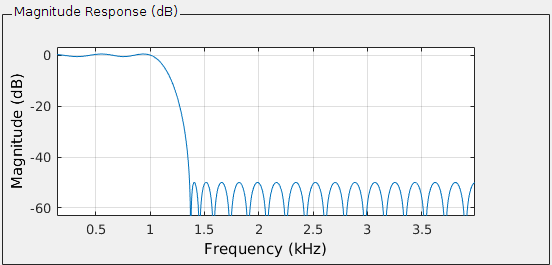
\includegraphics[width=0.32\textwidth]{lp_mag.png}
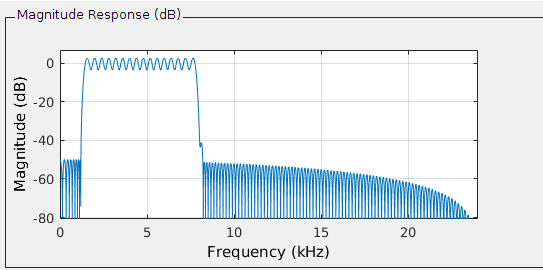
\includegraphics[width=0.32\textwidth]{bp_mag.png}
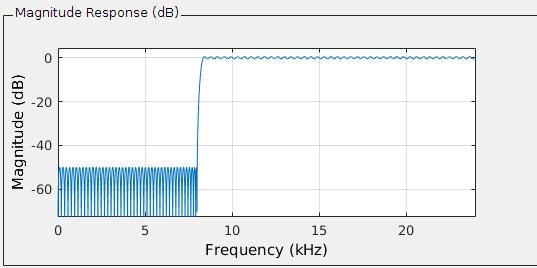
\includegraphics[width=0.32\textwidth]{hp_mag.png}
\end{center}

Besides the setting of band gain, the filter's quantization parameters should
be adjusted too. For a 16-bit fixed point processor like C5515, the word
length should be 16 bits, and Q15 format determines that the fraction length
needs to be 15 bits.

\subsection{Individual Band Gain Adjustment And Total Band Gain Calculation}
\label{sec:orgcb542f3}
According to the associativity property of the Convolution, the
implementation of multiple FIR filters of same order can be simplified into
one FIR filter whose coefficients are the combined coefficients.

$$y = x \ast h_1 \ast h_2 ... \ast h_n = x \ast \sum\limits_{i=1}^n h_i$$

\begin{listing}
\begin{verbatim}
void band_mix(){
  int i;
  for(i=0;i<TAPS;i++)
    band_coef_mixed[i] = band1_coef_changed[i] + band2_coef_changed[i] + band3_coef_changed[i];
}
\end{verbatim}
\centering
\caption{List 1: Band Coefficients Mixing}
\newline
\end{listing}

To perform the gain adjustment, each coefficient of the FIR filter needs to
multiply by the gain value. Since the gain is a constant value, the
multiplication operation can be performed directly on the filter's
coefficients.

$$F\{a \cdot H(v)\} = a \ast h(f)$$

To perform gain multiplication, each value of the gain needs to be hard coded
into hexadecimal for faster processing speed. Two Q15 format number's
multiplication will produce a Q30 format fixed-point number with 2 sign bits
ahead, hence it needs to be shifted to the right for 15 bits and chop the
redundant first sign bit.

\begin{listing}
\begin{verbatim}
for(i=0;i<TAPS;i++){
    band1_coef_changed[i]=(Int16)(((Int32)BAND1_COEF[i]*
                          (Int32)band_gain_hex[band1_gain_selection])>>15);
    band2_coef_changed[i]=(Int16)(((Int32)BAND2_COEF[i]*
                          (Int32)band_gain_hex[band2_gain_selection])>>15);
    band3_coef_changed[i]=(Int16)(((Int32)BAND3_COEF[i]*
                          (Int32)band_gain_hex[band3_gain_selection])>>15);
  }
\end{verbatim}
\centering
\caption{List 2: Gain Multiplication}
\newline
\end{listing}

\subsection{Button And FIR Filter}
\label{sec:orga0c9bd1}
The implementation of button is similar to what have done in
Ex.1 and Ex.2. For every running cycle, the main program is continue
monitoring the push button condition. Each time when a button is pushed, the
program checks the reading value to decide which button is pushed and react
correspondingly. In my program, button 1 controls the LED toggling and button
2 controls the gain adjustment.

\begin{listing}
\begin{verbatim}
btn_value = Get_Key_Human();
if (btn_value != NoKey){
  check_btn_push(btn_value);
}
\end{verbatim}
\centering
\caption{List 3: Check Button Condition}
\newline
\end{listing}

FIR function from the external library is used to read and write audio signal. 

\begin{listing}
\begin{verbatim}
fir(&x_right[0],&band_coef_mixed[0],&r_right[0],&dbuffer_right[0],1,TAPS);
fir(&x_left[0],&band_coef_mixed[0],&r_left[0],&dbuffer_left[0],1,TAPS);
\end{verbatim}
\centering
\caption{List 4: FIR Filter}
\newline
\end{listing}

\subsection{LCD Implementation}
\label{sec:org585c703}
This device includes a LCD Interface Display Driver (LIDD) controller, which
can be used for implementation of User Interface Menu Navigation. After
initialization of the LCD display, it require the clear function to clean the
screen. One can utilize the function 'OSD9616\(_{\text{send}}\)()' to print character or
string on the screen. The screen has top and bottom planes and each of them
needs to be set separately.

\begin{listing}
\begin{verbatim}
void printLetter(Uint8 font_array[4]){
  OSD9616_send(0x40,font_array[0]);
  OSD9616_send(0x40,font_array[1]);
  OSD9616_send(0x40,font_array[2]);
  OSD9616_send(0x40,font_array[3]);
  OSD9616_send(0x40,0x00);  // Line blank for space
}

void set_plane(int i){
  OSD9616_send(0x00,0x00);   // Set low column address
    OSD9616_send(0x00,0x10);   // Set high column address
  if (i == 0){
    OSD9616_send(0x00,0xb0); // Set page for page 0 to page 5
  } else if (i == 1){
    OSD9616_send(0x00,0xb1); // Set page for page 0 to page 5
  }
}
\end{verbatim}
\centering
\caption{List 5: LCD Setting And Printing}
\newline
\end{listing}

\subsection{Timer Interrupt And LED Blinking}
\label{sec:orga01479a}
To enable timer interrupt, IER0 and IFR0 have to be set. According to C5515
DSP System Guide, the CPU has only one interrupt flag that is shared among
the three timers. Since the interrupt flag is shared, software must have a
means of determining which timer instance caused the interrupt. Therefore,
the timer interrupt aggregation flag register (TIAFR) is a secondary flag
register that serves this purpose.

For the three general purpose timer, each of them has a count register
(TIMCNTn) which consists of two 16-bit words (TIMCNT1 and TIMCNT2) and a
period register (TIMPRDn) which also consists of two 16-bit words (TIMPRD1
and TIMPRD2). When the timer is set to start the contents of the TIMPRDn
register is loaded into the TIMCNT register and begins to count down. TCR is
the timer control register. When the LSB of TCR is set to 1, the timer starts
to count down.

\begin{listing}
\begin{verbatim}
void Reset();
interrupt void Timer_Handler()
{
  if (band_selection == 1){
    if (led1 == 0){
      USBSTK5515_ULED_on(1);
      led1 = 1;
    } else {
      USBSTK5515_ULED_off(1);
      led1 = 0;
    }
  }
  if (band_selection == 2){
    if (led2 == 0){
      USBSTK5515_ULED_on(2);
      led2 = 1;
    } else {
      USBSTK5515_ULED_off(2);
      led2 = 0;
    }
  }
  if (band_selection == 3){
    if (led3 == 0){
      USBSTK5515_ULED_on(3);
      led3 = 1;
    } else {
      USBSTK5515_ULED_off(3);
      led3 = 0;
    }
  }
  //printf("timer on %d\n", TIAFR);
}

Uint16 time_set;
Uint32 reset_loc = (Uint32)Reset;

void Timer_setup()
{

  //Set up Interrupt Vector Pointer Table
  IVPD = reset_loc >> 8;
  IVPH = reset_loc >> 8;

  *((Uint32*)((reset_loc + TINT)>>1)) = (Uint32)Timer_Handler; //Table points to our handler


  IER0 |= (1 << TINT_BIT);//enable interrupt
  IFR0 &= (1 << TINT_BIT);//clear the flag

  TCR0 = TIME_STOP;
  // Set total period 
  TPR0_1 = 0xFFFF; 
  TPR0_2 = time_offset + 4 * 16;
  // Set count down register
  TCR0_1 = 0x0001;
  TCR0_2 = 0x0000;

  // Clear Timer Interrupt Flag
  TIAFR = 0x0001;
  TCR0 = TIME_START_AUTOLOAD;
}
\end{verbatim}
\centering
\caption{List 6: Timer Interrupt And LED Blinking}
\newline
\end{listing}



\section{Conclusion}
\label{sec:orgdc3e846}
In summary, the design and the implementation meet the requirement of this
project. The Audio CODEC function block works compatibly with the button, LCD,
LED, and Timer Interrupt.


\section{Appendix}
\label{sec:org14fdefb}
Source Code: \url{https://github.com/seanhxx/schoolwork/tree/master/ee4413-dsp/assignment2}
\end{document}
